\section{Lexikalanalys}

Eftersom det skulle skapas ett språk för att skanna \textit{fak.c}, valdes att enbart det alfabet
som \textit{fak.c} använder. Språket togs fram genom att först analysera \textit{fak.c}.
\\ \textit{pas.l} användes som en mall för att utveckla språket för specifikt \textit{fak.c},
därav de tokens som fanns men var ej nödvändiga för \textit{fak.c} togs bort, och de som
behövdes laddes till. 

\begin{figure}[!h]
    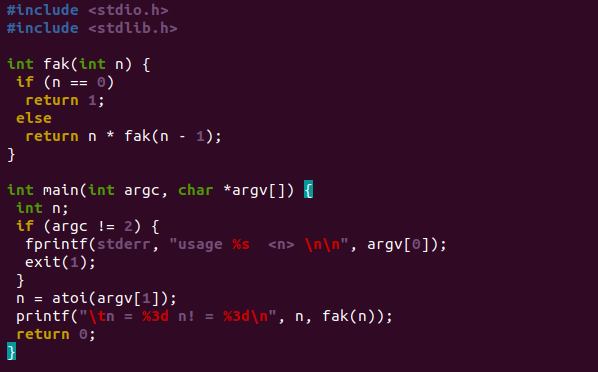
\includegraphics[width=\linewidth]{bilder/fak_c.png}
    \captionof{figure}{fak.c koden}
    \label{fig:fak_c}
\end{figure}


\begin{figure}[!h]
    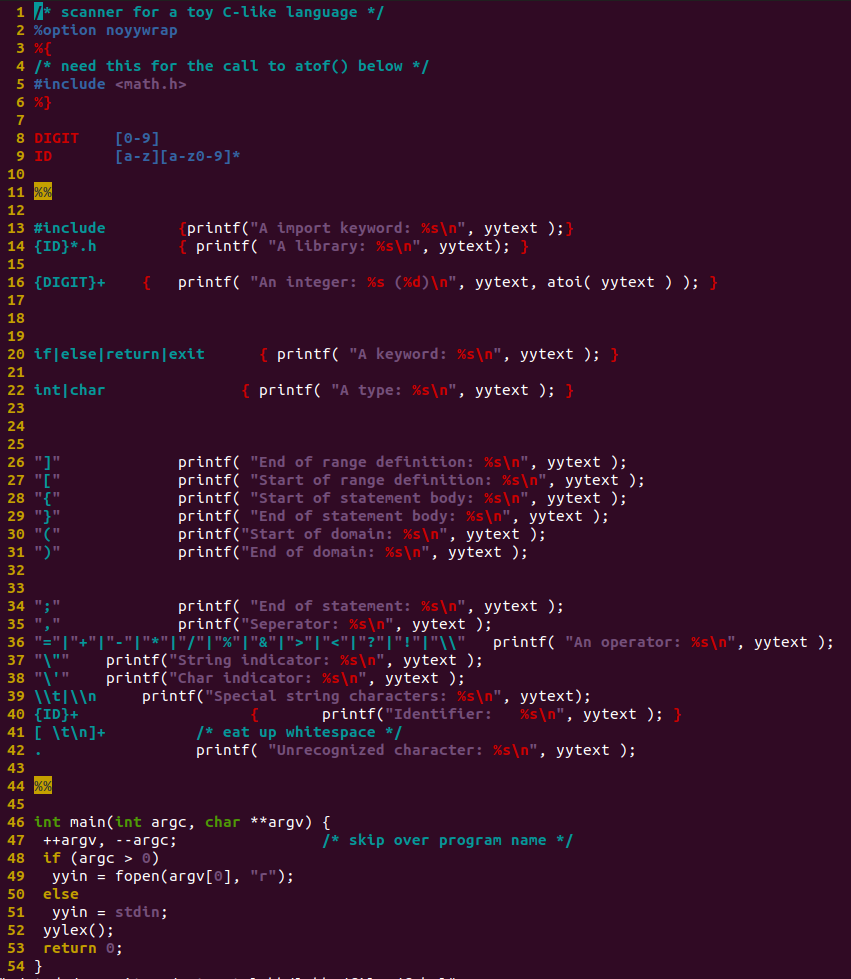
\includegraphics[width=\linewidth]{bilder/fak_l.png}
    \captionof{figure}{fak.l språket}
    \label{fig:fak_l}
\end{figure}


\begin{description}

\item[\textit{\#include}] I \textit{fak.l} är \textit{\#include} ett token för importering av biblotek. 

\item[\textit{{ID}*.h}] Med det fördefinerade \textit{ID} på rad 16 i
\textit{fak.l}, som säger att alla ord som är konstruerade med \textit{ID} och slutar
med \textit{.h}

\item[\textit{{DIGIT}+}] includerar alla heltal.

\item[\textit{if|else|return|exit}] Alla nyckel ord som uppstår i \textit{fak.c }
som existerar i programmerings språket c.

\item[\textit{int|char}] Typdeklarationerna som uppstår i \textit{fak.c}. 

\item[\textit{\\t|\\n}] Token för att känna igen speciella karaktärer i en sträng sekvens.

\item[\textit{rad 26-31}] Tokens som beskriver start och slut på gruppsekvenser för dem
operationer som använder sig av klammrar, måsvingar och paranteser.

\item[\textit{rad 34-49}] Beskriver tokens för diverse speciella karaktärer, deklarationer av
tillstånd separerare, operatorer för olika operationer samt deklarationer för strängar och
karaktärer.

\item[\textit{{ID}+}] För att skapa tokens åt identifierare används ett reguljärt uttryck för alla strängar som
består av enbart \textit{ID}.

\item[\textit{rad 41-42}] För resterande text finns det uttryck som känner igen tomt utrymme och
tecken som är inte inkluderat i språket.

\end{description}

 Tillsammans beskriver språket i filen \textit{fak.c}
